\documentclass[tikz]{standalone}
\usepackage{tikz}
\usetikzlibrary{arrows.meta, positioning, decorations.pathmorphing, decorations.markings, calc, shapes.geometric, fit}
\usepackage{amsmath,amssymb}

\definecolor{DarkSkyBlue}{RGB}{0, 51, 153}
\definecolor{domain1}{RGB}{180, 220, 255}
\definecolor{domain2}{RGB}{255, 220, 180}
\definecolor{elderpurple}{RGB}{160, 120, 200}

\begin{document}

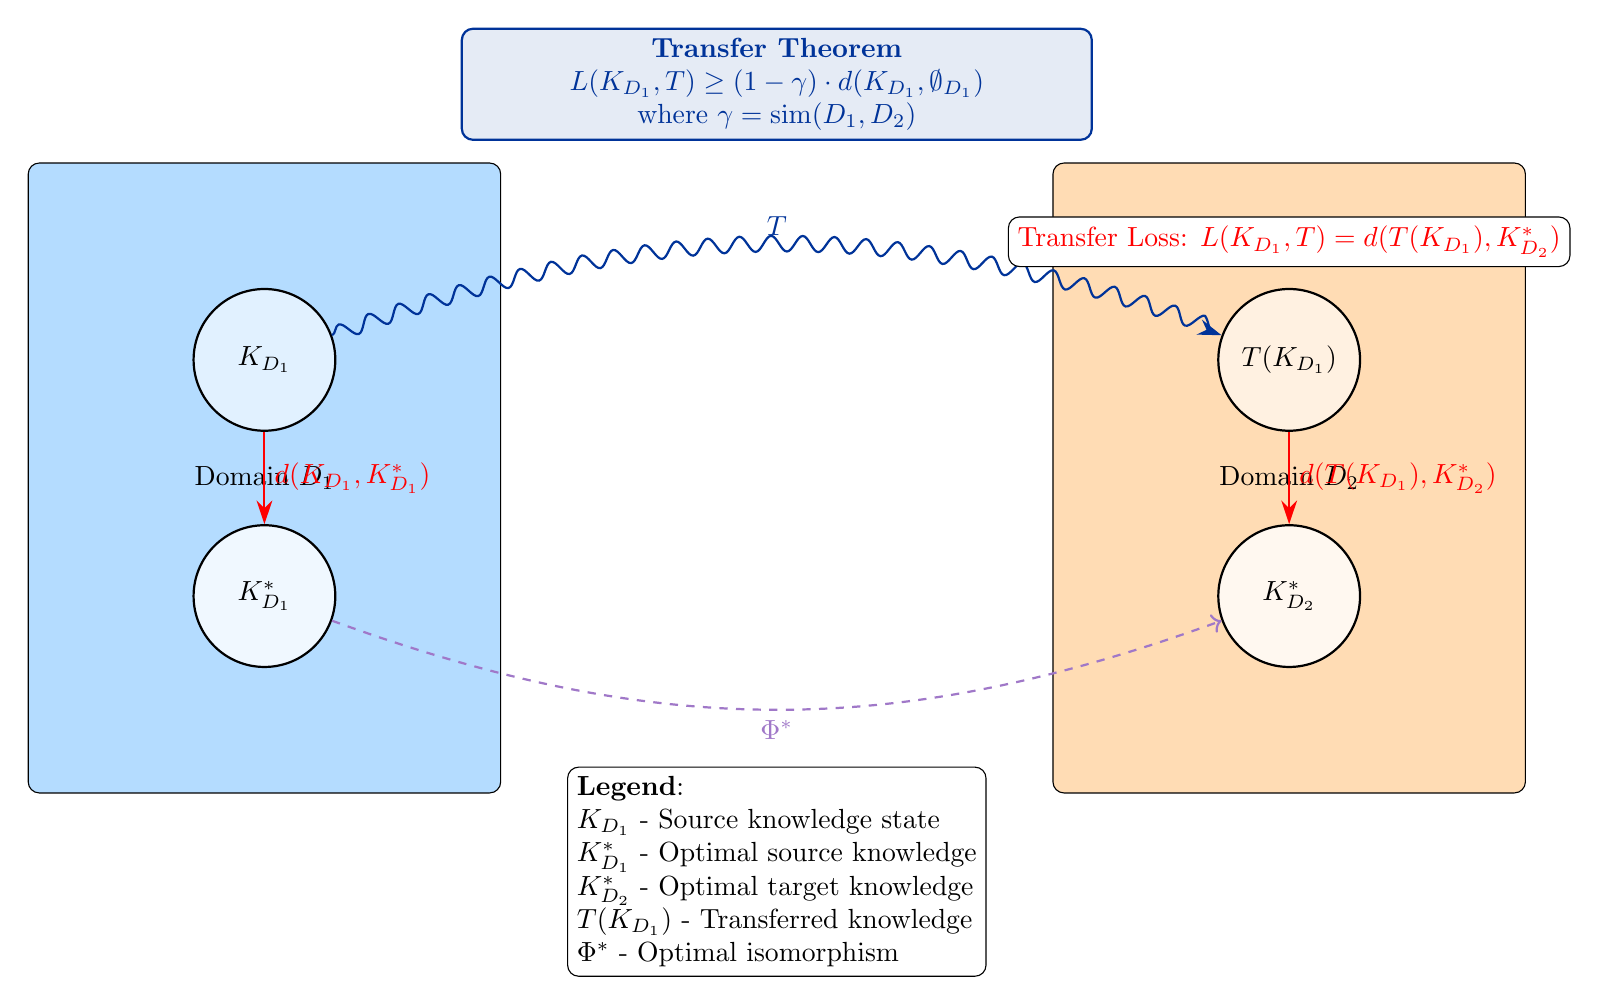
\begin{tikzpicture}[
    node distance=3cm,
    knowledge/.style={circle, draw, fill=white, minimum size=1.8cm, align=center},
    domain1/.style={draw, fill=domain1, rounded corners, minimum width=6cm, minimum height=8cm, align=center},
    domain2/.style={draw, fill=domain2, rounded corners, minimum width=6cm, minimum height=8cm, align=center},
    arrow/.style={-{Stealth[length=3mm, width=2mm]}, line width=0.7pt},
    dasharrow/.style={dashed, ->, line width=0.5pt},
    distortion/.style={decorate, decoration={snake, amplitude=1mm, segment length=4mm}}
]

% Domains
\node[domain1] (d1) {Domain $D_1$};
\node[domain2, right=7cm of d1] (d2) {Domain $D_2$};

% Knowledge states
\node[knowledge, fill=domain1!40!white, thick] (k1) at ($(d1) + (0,1.5)$) {$K_{D_1}$};
\node[knowledge, fill=domain1!20!white, thick] (k1star) at ($(d1) + (0,-1.5)$) {$K_{D_1}^*$};

\node[knowledge, fill=domain2!20!white, thick] (k2star) at ($(d2) + (0,-1.5)$) {$K_{D_2}^*$};
\node[knowledge, fill=domain2!40!white, thick] (k2) at ($(d2) + (0,1.5)$) {$T(K_{D_1})$};

% Distance markers
\draw[arrow, red] (k1) -- (k1star) node[midway, right] {$d(K_{D_1}, K_{D_1}^*)$};
\draw[arrow, red] (k2) -- (k2star) node[midway, right] {$d(T(K_{D_1}), K_{D_2}^*)$};

% Transfer operation
\draw[arrow, thick, distortion, DarkSkyBlue] (k1) to[bend left=20] node[midway, above] {$T$} (k2);

% Isomorphism
\draw[dasharrow, thick, elderpurple] (k1star) to[bend right=20] node[midway, below] {$\Phi^*$} (k2star);

% Loss indicator
\node[draw, fill=white, rounded corners, text=red] at ($(d2) + (0,3)$) {Transfer Loss: $L(K_{D_1}, T) = d(T(K_{D_1}), K_{D_2}^*)$};

% Legend
\node[rectangle, draw, rounded corners, fill=white, minimum width=5cm, minimum height=2.5cm, align=left] at ($(d1)!0.5!(d2) + (0,-5)$) {
    \textbf{Legend}:\\
    $K_{D_1}$ - Source knowledge state\\
    $K_{D_1}^*$ - Optimal source knowledge\\
    $K_{D_2}^*$ - Optimal target knowledge\\
    $T(K_{D_1})$ - Transferred knowledge\\
    $\Phi^*$ - Optimal isomorphism
};

% Bound
\node[rectangle, draw, DarkSkyBlue, thick, rounded corners, fill=white!90!DarkSkyBlue, minimum width=8cm, align=center] at ($(d1)!0.5!(d2) + (0,5)$) {
    \textbf{Transfer Theorem}\\
    $L(K_{D_1}, T) \geq (1 - \gamma) \cdot d(K_{D_1}, \emptyset_{D_1})$\\
    where $\gamma = \text{sim}(D_1, D_2)$
};

\end{tikzpicture}

\end{document}